\documentclass[a4paper, 14pt]{extreport}
\usepackage[left=15mm, top=20mm, right=15mm, bottom=30mm, nohead]{geometry}

\input{basic-tex-config/preamble.tex}
\usepackage{tikz}
\usepackage{pgfplots}
\pgfplotsset{compat=1.11}
\newtheorem{definition}{Определение}
\title{Суммирование точек на эллиптической кривой}
\date{\today}
\author{Плотников Антон. А4101.}

\begin{document}
\maketitle

\section*{Определение}
\begin{definition}
    Рассмотрим конечное поле $F_q, q = p^k$ с характеристикой $p \geq 2$.

    Тогда эллиптической кривой над полем $F_q$ называется множество точек
    $(x, y) \in F_q \oplus F_q$, удовлетворяющих уравнению Вейерштрасса:
    \begin{gather}\label{eq:full_weier}
        y^2 + ay + b = x^3 + cx^2 + dx + e,
    \end{gather}
    вместе со специальной точкой, обозначающейся символом $\infty$ и называемая
    точкой в бесконечности.

    Если $p \geq 3$, то уравнение~\ref{eq:full_weier} может быть преобразовано
    в сокращенное уравнение Вейерштрасса:
    \begin{gather}\label{eq:short_weier}
        y^2=x^3+ax+b,
    \end{gather}
    где $a, b \in F_q$.
\end{definition}

Важными характеристиками эллиптической кривой являются её дискриминант $\Delta$
и инвариант $j$:
\begin{gather}
    \Delta = -16(4a^3 + 27b^2) \qquad j = \frac{1728{(4a)}^3}{\delta}
\end{gather}
На множестве точек $E$ \emph{неособой} эллиптической кривой (детерминант
$\Delta$, которой не равен нулю) можно определить групповую операцию
суммирования $+$. Нулем будет этой группы является точка $\infty$, а обратным
элементом по сложению к точке $P = (x, y) \in E$ будет являться точка $-P = (x,
-y)$.

\section*{Суммирование точек на эллиптической кривой}

Проведем прямую через пару произвольных точек $P$ и $Q$ прямую $L$ до
пересечения с третьей точкой $R$, такая точка обязательно найдется, т.к.
пересечение произвольной прямой с эллиптической кривой имеет либо одну либо 3
точки пересечения.

Определим сумму трех точек $P(x_p, y_p)$, $Q(x_q, y_q)$ и $R(x_r, y_r)$ равной
нулю:
\begin{gather}
    P+Q+R=\infty,
\end{gather}
тогда $P+Q=-R$.

Для вычисления координаты точки $S(x_s, y_s) = P + Q$ найдем параметры прямой
$L$: $y=\lambda x + d$:
\begin{gather}
    y = \frac{y_q - y_p}{x_q - x_p},\,d=y_p - \lambda x_p.
\end{gather}

Подставляя выражение для $L$ в уравнение~\ref{eq:full_weier} получим:
\begin{gather}
    x^3 + cx^2 + ax + b - {(\lambda x + d)}^2 = 0.
\end{gather}
Сумма координат $x_p + x_q + x_s$ должна быть равна коэффициенту при $x^2$,
взятому с противоположным знаком:
\begin{gather}
    x_p + x_q + x_s = \lambda^2 - c = {\left(\frac{y_q - y_p}{x_q -
    x_r}\right)}^2 - c,
\end{gather}
отсюда получим формулу для координат суммы:
\begin{gather}
    \begin{cases}
        x_s = \lambda^2-x_p-x_q-c\\
        y_s = \lambda(x_p-x_q) - y_p = \lambda(2x_p+x_q-\lambda^2+c) - y_p
    \end{cases}.
\end{gather}

Если точки $P$ и $Q$ совпадают, то угловой коэффициент прямой $L$ можно найти
дифференцируя уравнение~\ref{eq:full_weier} по $x$.

\begin{figure}
\centering
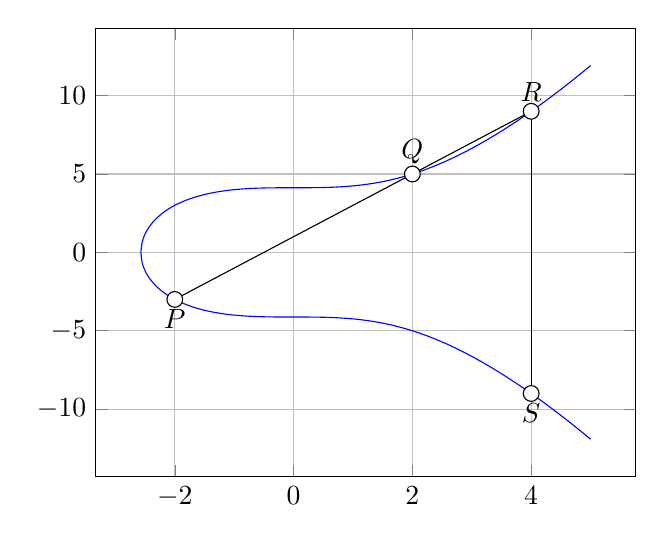
\begin{tikzpicture}
    \begin{axis}[samples=400,domain=-2.571281:5,grid=both]
        \addplot[blue] {sqrt(x^3+17)};
        \addplot[blue] {-sqrt(x^3+17)};
        \coordinate[label={-90:$P$}] (P) at (axis cs:-2,-3);
        \coordinate[label={90:$R$}] (R) at (axis cs:4,9);
        \coordinate[label={90:$Q$}] (Q) at (axis cs:2,5);
        \coordinate[label={-90:$S$}] (S) at (axis cs:4,-9);
        \draw (P) -- (Q) -- (R);
        \draw (R) -- (S);
        \draw[fill=white] (P) circle (1mm);
        \draw[fill=white] (Q) circle (1mm);
        \draw[fill=white] (R) circle (1mm);
        \draw[fill=white] (S) circle (1mm);
    \end{axis}
\end{tikzpicture}
\caption{Геометрическая интерпретация операции суммирования}
\end{figure}

\end{document}
